\section{Methodology}

%\subsection{Operational Pipeline for News Data Collection}
\subsection{Overview of the Proposed Method}

The proposed method is designed to streamline the risk data collection and identification from news sources for users. This section details the proposed method as an operational pipeline from the perspective of a user using the system.

The proposed method, as illustrated in Fig.~\ref{fig:pipeline}, automates the summarization, identification, and updating of disruption database based on the URLs submitted by users. The process is designed to be intuitive and user-friendly, allowing users to efficiently collect and analyze the risk data.

\begin{figure*}[ht!]
\centering
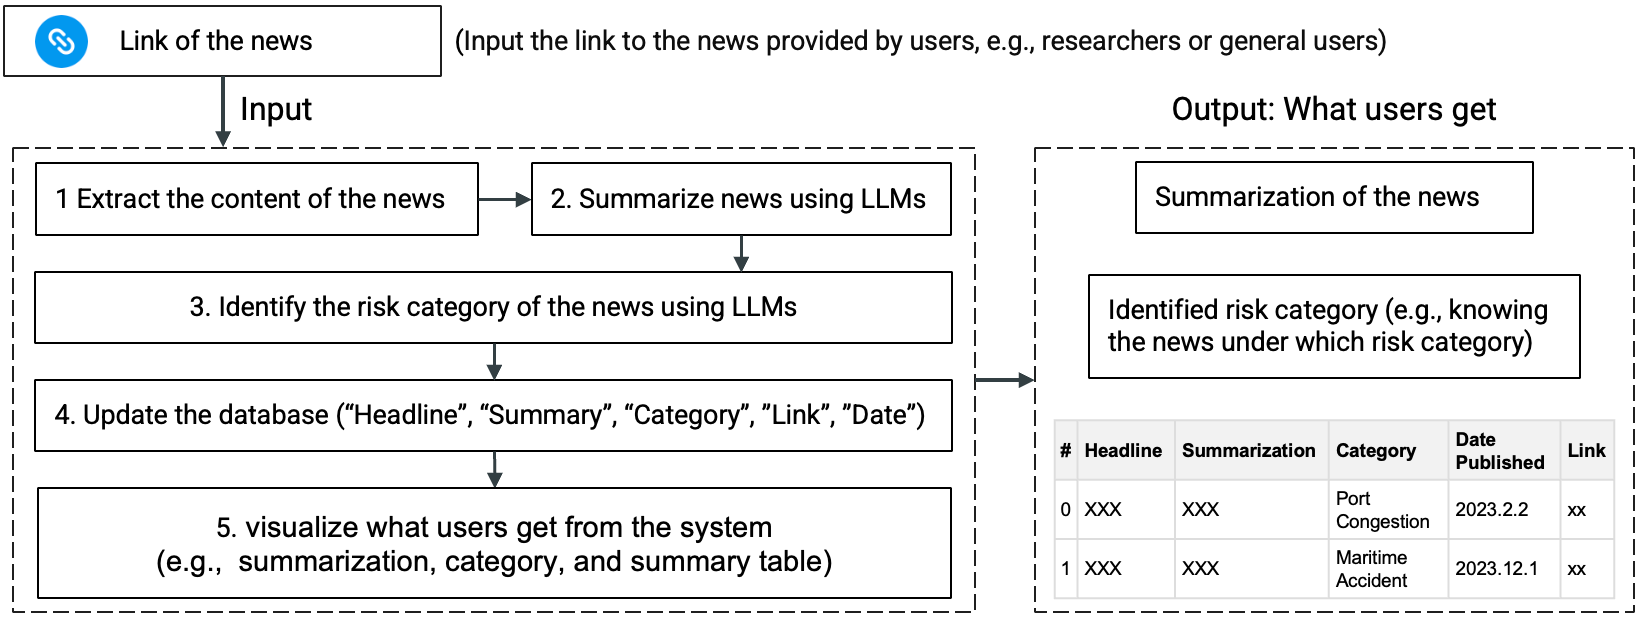
\includegraphics[width=0.66\textwidth]{figures/pipeline.png}
\caption{Schematic Overview of the Proposed Method: Operational Pipeline for Risk Data Collection and Identification from News Sources. This figure illustrates the step-by-step process of the automated risk data collection and identification system, from URL submission by users to the generation of a summary table. Key steps include: 1. Extract the content of the news, 2.Summarize the news using LLMs, 3. Identify the risk category of the news using LLMs, 4. Update the database, and 5. Visualize what users get from the system. 
%The pipeline demonstrates the integration of LLM capabilities with traditional database operations to streamline maritime risk data analysis.
}
\label{fig:pipeline}
\end{figure*}


As shown in Fig.~\ref{fig:pipeline}, the interaction begins when a user submits the URL of a disruption event. In the first key step (Step 1), the system extracts the content of the news and checks whether the event already exists in the database. If the event is new, the model will proceed with the following steps: summarizing the news, identifying the risk category, updating the database with the key elements, and presenting a summary of the information to users through visualization. This summary provides users with a quick overview of the news article’s content.
The prompt used for summarizing by LLM is shown in Listing \ref{lst:summary-prompt}.

\vspace{1.5\baselineskip}
\begin{lstlisting}[caption={Prompt for LLM Summarization}, 
                   label={lst:summary-prompt}, 
                   breaklines=true, 
                   basicstyle=\footnotesize\ttfamily, 
                   xleftmargin=0pt, 
                   framexleftmargin=0pt, 
                   framesep=0pt, 
                   aboveskip=0pt, 
                   belowskip=0pt, 
                   showspaces=false, 
                   showstringspaces=false,
                   keepspaces=true,
                   breakindent=0pt]
Summarize the following article in about 70 words, focusing on what happened, where it happened, and the consequences (economic loss, environmental impact, etc.): {article}
\end{lstlisting}

Following the summarization (Step 2: Summarize the news using LLMs), the model identifies the risk category (Step 3: Identify the risk category of the news using LLMs). The results from both steps are used in the subsequent step to better organize the data into meaningful segments, enhancing usability for users. For this research, we evaluated the performance of traditional ML models and modern Large Language Models (GPT-4, Llama-3.1). Our comparative analysis focused on key performance metrics, such as accuracy and the ability to discern nuanced distinctions across diverse news topics.

Once the identification (Step 3) is complete, Step 4: Update the database will be conducted. This step involves updating and enriching the database by adding detailed records, including the event's headline, summary, risk category, URL link, and publication date. To further support user-friendly efforts, the model identifies and ranks related news events within the same category based on their recency. This functionality enables users to quickly access the most current and relevant information within their area of interest.

For enhanced risk data presentation, the system is designed to visualize what users get from it (Step 5). The system not only visualizes the summarization of the news and the identified risk category but also generates a summary table that distills the collected data into an easy-to-digest format, presenting key information such as headlines, summaries, categories, and publication dates. 
%For instance, if a user is analyzing the impact of earthquakes, they can discover recent earthquake events and explore related articles. The model retrieves related articles categorized under 'earthquake,' prioritizing those with greater recency. This ensures that users have access to the most up-to-date and contextually relevant information, as older articles may not reflect current economic conditions, building standards, or environmental policies.

\subsection{Comparative Study of GMRID Identification: Traditional Models vs. LLMs}

In this study, we evaluated the performance of both traditional classification models and modern Large Language Models (LLMs) such as GPT-4o and Llama-3.1. Our comparative analysis focused on key performance metrics, including accuracy and the ability to distinguish nuanced differences across diverse news topics.

We implemented five traditional machine learning models---Naive Bayes, Logistic Regression, Support Vector Machine (SVM), Random Forest, and K-Nearest Neighbors---using the scikit-learn library\footnote{\url{https://scikit-learn.org/}}. Training, evaluation, and hyper-parameter tuning were conducted with both the GMRID v1 and v2 datasets.

In addition to traditional models, we employed OpenAI’s GPT-4o and GPT-4o-mini, as well as Meta's Llama-3.1-8B and Llama-3.1-70B models, for classification tasks. The dataset was split into two subsets, with 80\% used for training and 20\% reserved for testing.

To enable the LLMs to perform classification, we utilized few-shot prompting techniques. The system prompt template used for this classification is provided in Listing \ref{lst:llm-classification-prompt}.

\vspace{2.0\baselineskip}
\begin{lstlisting}[caption={Prompt for LLM Classification}, 
                   label={lst:llm-classification-prompt}, 
                   breaklines=true, 
                   basicstyle=\scriptsize\ttfamily, 
                   xleftmargin=0pt, 
                   framexleftmargin=0pt, 
                   framesep=0pt, 
                   aboveskip=0pt, 
                   belowskip=0pt, 
                   showspaces=false, 
                   showstringspaces=false,
                   keepspaces=true,
                   breakindent=0pt]
Task: You are a classifier. Your objective is to analyze the given input and assign it to one of the predefined categories: {categories}. Evaluate the content carefully and use the defining characteristics of each category to ensure an accurate classification.

Guidelines:
1. Understand the Categories: Familiarize yourself with the specific attributes of each category by referring to the category descriptions provided in the JSON: {categories_json}.
2. Contextual Analysis: Consider the broader context of the input. If an input could potentially fit into multiple categories, select the one that best reflects its primary intent or focus.
3. Handling Ambiguity: For ambiguous inputs or those that do not clearly align with any category, choose the category that most closely matches the content provided.
4. Ensure Accuracy and Consistency: Strive for consistent and accurate classifications. Avoid arbitrary or random assignments.
5. Provide Feedback: If the input cannot be classified into any of the given categories, return "Others".
{exemplars}
Output Format: Return only the name of the category that the input belongs to. If uncertain, respond with "Others".
\end{lstlisting}

The system prompt template is designed as a versatile tool for text classification. In our study, the placeholders were populated with the following specific data:

\begin{itemize}
    \item \texttt{\{categories\}}: A list of primary categories, as shown in Table \ref{tab:event_categories}.
    \item \texttt{\{categories\_json\}}: A JSON structure mapping primary categories to initial unstructured categories, as detailed in Table \ref{tab:event_categories}.
    \item \texttt{\{exemplars\}}: For zero-shot classification, this field is left empty; for few-shot classification, exemplars are retrieved from the GMRID training set and formatted as shown in Listing \ref{lst:exemplars-prompt}.
\end{itemize}

\begin{lstlisting}[caption={Exemplars Used in Few-Shot Prompting}, 
                   label={lst:exemplars-prompt}, 
                   breaklines=true, 
                   basicstyle=\scriptsize\ttfamily, 
                   xleftmargin=0pt, 
                   framexleftmargin=0pt, 
                   framesep=0pt, 
                   aboveskip=0pt, 
                   belowskip=0pt, 
                   showspaces=false, 
                   showstringspaces=false,
                   keepspaces=true,
                   breakindent=0pt]
Example Inputs and Outputs:
- Input: local source reported operation at pier 1 and 2 of the container terminal at port of durban was suspended due to strong winds ...
- Classification: Weather
... 
\end{lstlisting}

%the Port of Durban was suspended due to strong winds on December 27 at 18:50 local time, resuming at 23:10 the same day. Pier 2 terminal operations were halted at 19:30 and resumed at 20:35 respectively.

Using the above prompting techniques, the evaluation of GPT-4o and GPT-4o-mini models was conducted via the OpenAI API\footnote{\url{https://platform.openai.com/docs/overview}}, while the evaluation of Llama-3.1 models was performed on Nvidia L40 GPUs using the HuggingFace Transformers library\footnote{\url{https://huggingface.co/docs/transformers/en/index}}.

\subsection{Evaluation Metrics}

To evaluate the performance of each model, we calculated predictive accuracy on the held-out test data using the weighted F1 score. This metric provides an overall measure of the model’s performance by taking into account both precision and recall, giving a balanced view of the model's ability to correctly classify data.

During the evaluation process, we observed that the Large Language Models (LLMs) occasionally produced outputs that did not correspond to any valid category labels defined in Table \ref{tab:event_categories}. Table \ref{tab:classification_results} presents a sample of classification results produced by the Llama-3.1-8B model, using different numbers of shots (0, 1, 3, 5, and 10).

\begin{table}[ht]
\caption{Sample Classification Results from Llama-3.1-8B Model Using Different Numbers of Shots. This table presents the outputs of the Llama-3.1-8B model for a single input across varying numbers of shots (0, 1, 3, 5, and 10). It illustrates the model's tendency to produce lengthy explanations and justifications, particularly with fewer shots, highlighting the challenge of generating concise, valid category labels consistently.}
\centering
\setlength{\tabcolsep}{6pt} % Adjust column padding
\renewcommand{\arraystretch}{1.2} % Adjust row height
\begin{tabularx}{.49\textwidth}{|>{\raggedright\arraybackslash\hspace{0pt}}p{1.2cm}|>{\raggedright\arraybackslash\hspace{0pt}}X|}
\hline
\textbf{Details (Cleaned)} & thursday reported operation u.s. air cargo company like fedex ups affected novel coronavirus covid-19 quarantine testing measure imposed 
official china report chinese official told flight crew would required quarantine ... \\
\hline
\textbf{Ground Truth} & Administrative Issue \\
\hline
\textbf{0-shot(s) Result} & Based on the provided input, the category that best fits the content is 'Administrative Issue'. The input discusses ... \\
\hline
\textbf{1-shot(s) Result} & Based on the provided input, the classification is: Others. \textit{Reasoning}: The input discusses the impact of COVID-19 quarantine measures on air cargo operations in China ... \\
\hline
\textbf{3-shot(s) Result} & Based on the input, the classification is: Administrative Issue. \\
\hline
\textbf{5-shot(s) Result} & Based on the input, the classification is: Administrative Issue. \\
\hline
\textbf{10-shot(s) Result} & Administrative Issue \\
\hline
\end{tabularx}
\label{tab:classification_results}
\end{table}

Based on the results in Table \ref{tab:classification_results}, we observe that the Llama-3.1-8B model correctly classifies the input as 'Administrative Issue' when given 10 shots. However, in other cases, the model produces lengthy explanations and justifications for its classifications, resulting in outputs that do not directly align with the predefined categories. These outputs are deemed "invalid categories" and cannot be directly used for performance calculations. To address this issue, we developed a post-processing function to extract valid categories from the LLM outputs, ensuring accurate computation of the F1 scores.

We also noted that "invalid categories" were more frequent in the smaller models, which often lack the capability to strictly follow instructions, undermining the reliability of their performance in classification tasks.

To further quantify this issue, we introduced a new metric called the Ratio of Valid Categories ($RVC$):

\begin{equation}
\text{$RVC$} = \frac{\text{Number of Valid Categories}}{\text{Total Number of Entries}}
\end{equation}

A “valid category” is any output generated by the model that matches the predefined set of category labels. 
This metric, $RVC$, provides insight into each model's reliability in producing valid classifications. A higher ratio indicates greater consistency in assigning entries to valid categories, which is crucial in classification tasks where the accuracy of labels directly affects the model's effectiveness.
